
\section{Descriptive Analytics}
\label{sec:DescriptiveAnalytics}

\subsection{Temporal Demand Patterns and Seasonality}
\label{subsec:TempDemand}

The Usage and Utilization metrics are introduced on a monthly, daily and hourly basis and further contrasted with temperature and precip (rain/snow) rate. The Usage of bike fleet describes how many rentals are started on the respective aggregation level. The Utilization rate is calculated by the ratio (x/n), where x describes the number of unique bikes, based on their bike ids, that have been used at least once and n is assigned to the total number of unique bikes.
The summer months record the highest usage and utilization numbers and the winter months the lowest numbers. This is referred to as annual seasonality, attributed to the seasons and can be observed in \hyperref[heatmap]{Figure 1}, \hyperref[fleetUsageYear]{Figure 2} and \hyperref[fleetUtilizationYear]{Figure 3}. The positive correlation with temperature values supports this observation. Furthermore, a daily pattern can be seen and can be attributed to commuters. People ride to work in the morning hours and return in the afternoon. Afternoon trip numbers are higher than morning trips, so it is suspected that additional leisure trips begin after work.
Finally, the negative correlation between rainfall and usage or utilization should be mentioned, visualized in \hyperref[fleetUtilizationYear]{Figure 4} and Appendix. High rainfall rates indicate low utilization rates or usage numbers and vice versa.

\begin{figure}[H]
    \centering
    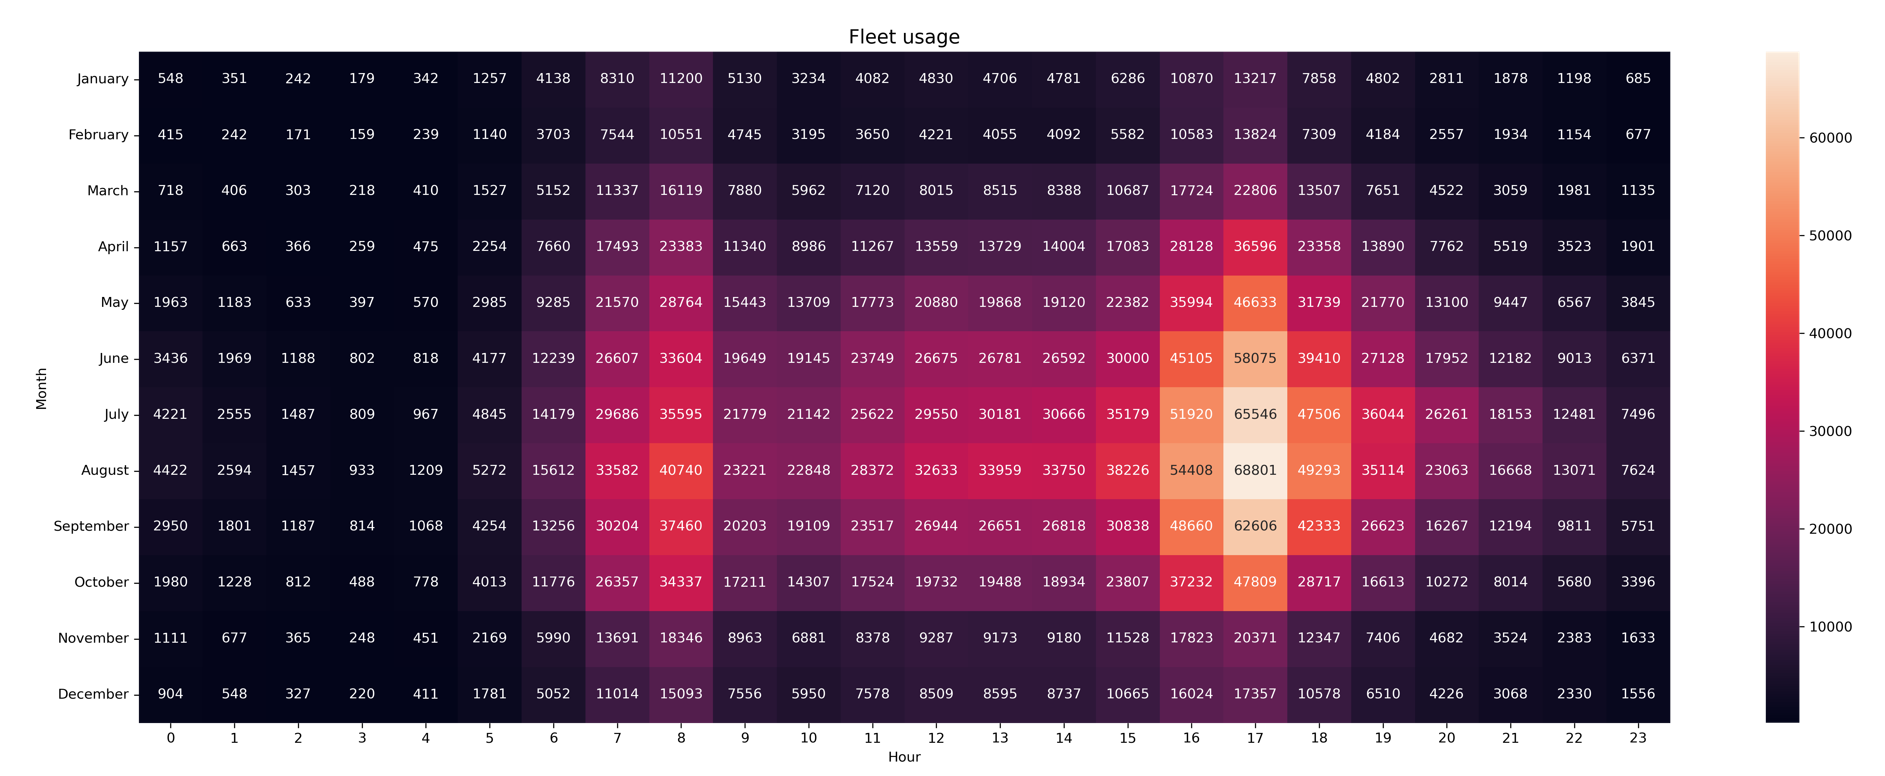
\includegraphics[width=1\linewidth]{./Figures/Usage_Heatmap.png}
    \caption{Fleet Usage}
    \label{heatmap}
\end{figure}

\begin{figure}[H]
    \centering
    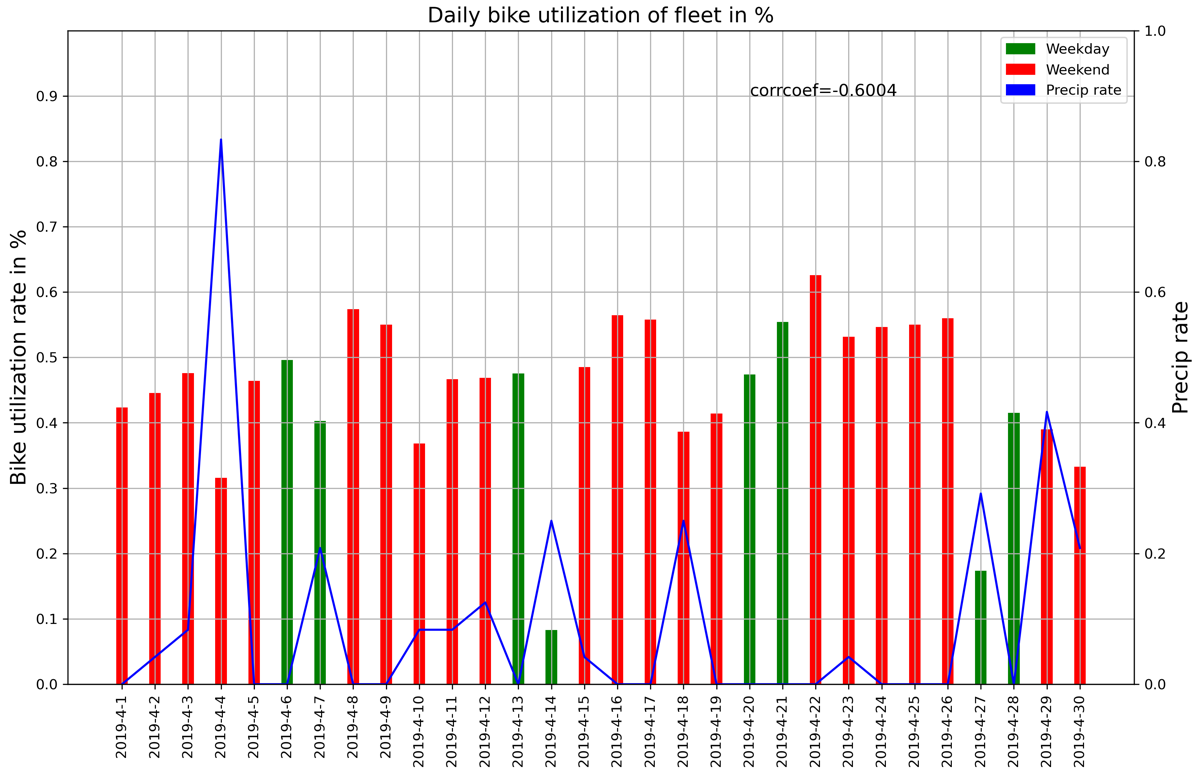
\includegraphics[width=0.7\linewidth]{./Figures/dailyBikeUtilizationApril.png}
    \caption{Daily Bike Utilization of fleet for April}
    \label{dailyBikeUtilizationApril}
\end{figure}

\subsection{Geopraphical Demand Patterns and Top X Stations}
\label{subsec:GeoDemand}

The following section deals with the investigation of the utilization of the individual stations. Several metrics were used to investigate the stations under different perspectives. The first metric we took was to measure the total sum of rides that start and end at each station and to plot the most heavily utilized stations under this definition. 

\begin{figure}[H]
    \centering
    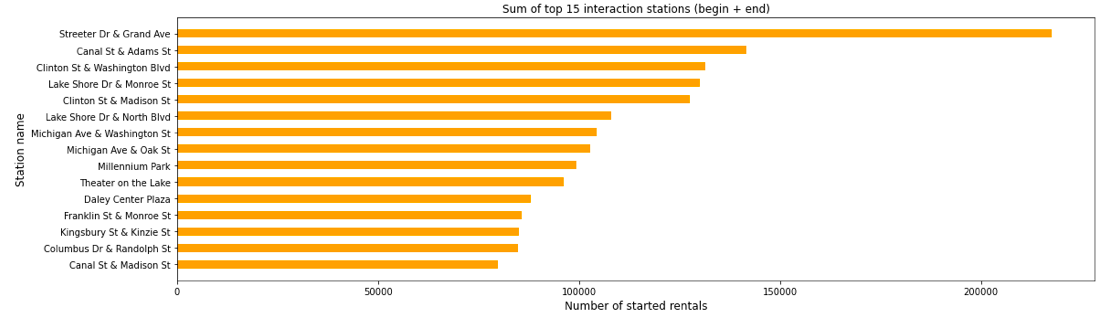
\includegraphics[width=1\linewidth]{./Figures/GeoAbb1.png}
    \caption{Top 15 statitions in terms of starting rides}
    \label{fig1}
\end{figure}


\hyperref[fig1]{Figure 1} illustrates the respective top 15 stations. As can be seen in the plot, the first five stations have a significant lead compared to the place 6 to 15. As a dashboard user, these stations can be seen as most important and should be monitored carefully to avoid longer maintenance. 
Building further upon those 15 stations, a highly skewed distribution of station interactions can be seen in \hyperref[fig4]{Figure 2}. 

\begin{figure}[H]
    \centering
    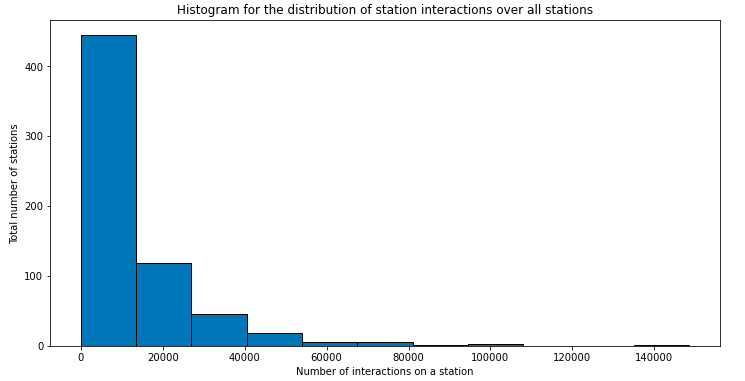
\includegraphics[width=0.7\linewidth]{./Figures/GeoAbb4.png}
    \caption{Histogram for the distribution of station interactions over all stations}
    \label{fig4}
\end{figure}

Most stations only have limited number of interactions. However, the top 50 stations already account for one third of the overall interactions. Also, the 0.75-quantile is very meaningful, stating that 75 percent of all stations have 16,850 or less interactions. Nevertheless, one should not diminish the importance of these stations, as 31 percent of all interactions are represented by them, stating that also the smaller stations are vital for daily business.
Another perspective was taken in \hyperref[fig4]{Figure 3}.

\begin{figure}[H]
    \centering
    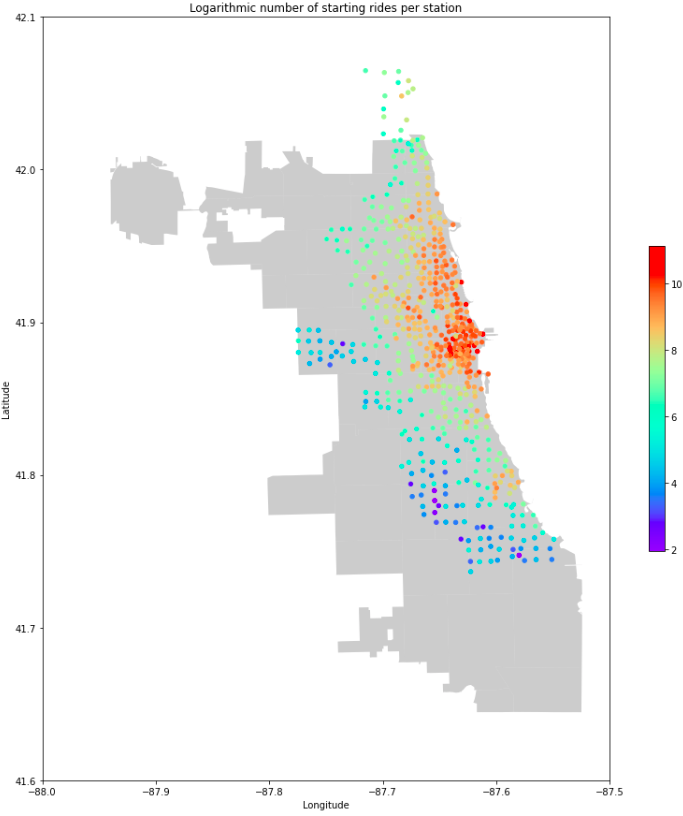
\includegraphics[width=0.6\linewidth]{./Figures/GeoAbb9.png}
    \caption{Logarithmic number of starting rides per station}
    \label{fig9}
\end{figure}


Here, the logarithmic number of starting rides per station is plotted. It can be easily seen that most of the rides start in the center of Chicago and along the coast, whilst moving to the outskirts of the city decreases the density of rides. The data can thus be clustered into three areas: The core of the city, with the most dense network, then the surroundings of that core that are still centrally located in Chicago and lastly, the outskirts, where only minor amounts of rides are started. We will refer to this structure as "three-ring structure" for the rest of this assignment.  


\subsection{KPI 1: RPUB (Rides Per Unique Bike)}
\label{subsec:KPI1}

The first KPI scrutinizes the number of trips per unique bicycle. The definition of "unique bicycle" is defined as follows: All unique bikes used per each day. The KPI is derived from an article by Sven Boor (2019) and an article by Yanocha, Mason, Patlán, Benicchio et al. (2018), although we adapted the KPI by also calculating hourly values, not only daily ones, in order to fulfill the task. The first insight that can be derived is that a clear seasonality can be exhibited with the highest values during summer and the lowest during winter \hyperref[kpi1abb1]{Figure X}.

\begin{figure}[H]
    \centering
    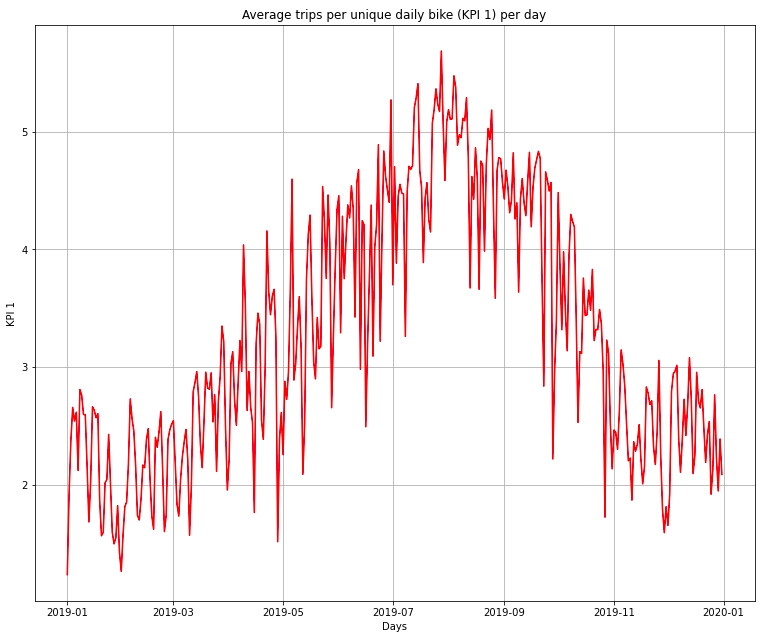
\includegraphics[width=0.7\linewidth]{./Figures/kpi1abb1.png}
    \caption{Average trips per unique daily bike (KPI 1) per day}
    \label{kpi1abb1}
\end{figure}

RPUB based on unique daily bikes always lies within the interval defined by Boor (2019) of 4-8 trips per bike. During summer, it averages around a value of 5, which is fine, however during winter, spring and autumn, it falls below the lower boundary of 4 defined by Boor (2019). This could indicate that the number of bikes during winter is too high.

\begin{figure}[H]
   \centering
    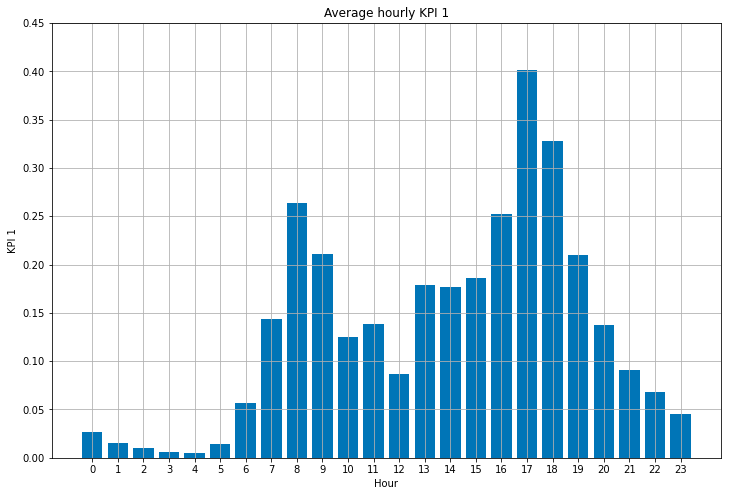
\includegraphics[width=0.7\linewidth]{./Figures/kpi1abb3.png}
    \caption{Average hourly KPI 1}
    \label{kpi1abb3}
\end{figure}

When looking at the hourly RPUB values averaged over the entire year \hyperref[kpi1abb3]{Figure X}, a very explicit commuter pattern can be observed, as the values peak at around 8 and 17 o' clock. Interestingly, at 5 o'clock, the KPI stands at around 0.4, which is more than twice as high than the average monthly value in July, the most "active" month. A bike at that time performs around 0.4 rides per hour. Thus, commuting activity has a tremendous impact on the utilization of the divyy system, much more than monthly seasonality.
Comparing weekend and weekdays hourly \hyperref[kpi1abb5]{Figure X}, it becomes clear that the weekend RPUB values are not higher or lower than the weekday ones, except for the situation during noon and at around 9/17 o' clock. Thus, it can again be reasoned that commuting is a significant driver of the divyy bike system and peak around noon due to leisure activities. As the influence of the weather data was insignificant, it can be consulted in the \hyperref[APP1]{Appendix}.

\begin{figure}[H]
   \centering
    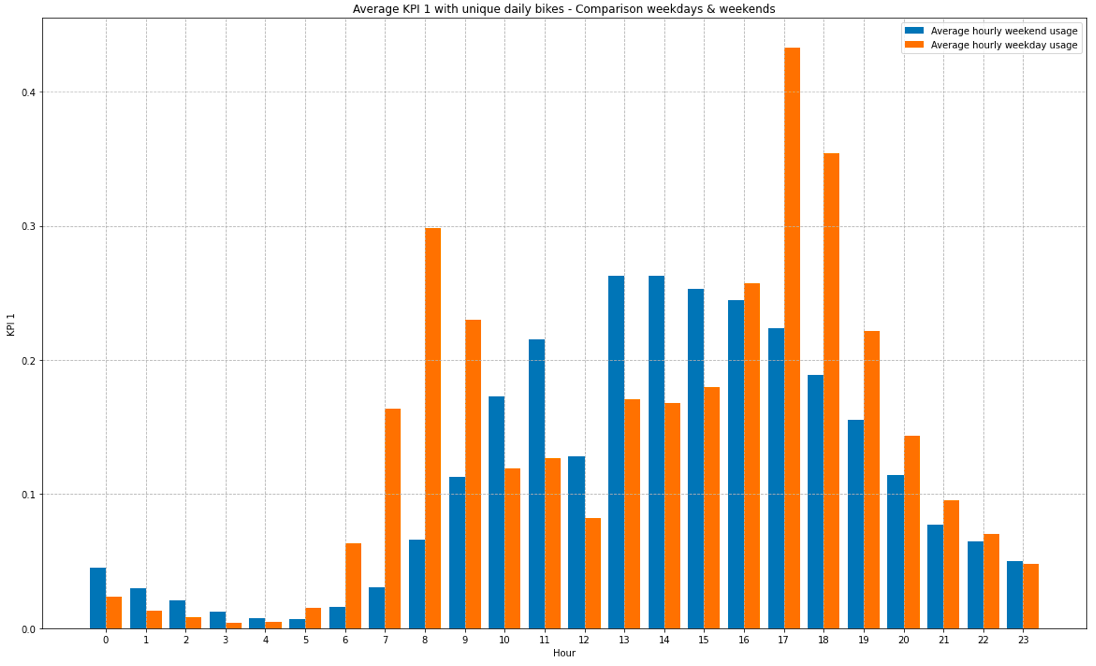
\includegraphics[width=0.7\linewidth]{./Figures/kpi1abb5.png}
    \caption{Average KPI 1 with unique daily bikes - Comparison weekdays & weekends}
    \label{kpi1abb5}
\end{figure}

\subsection{KPI 2: Demand-Capacity}
\label{subsec:KPI2}

This KPI is related to "coverage". The KPI should investigate whether the distribution and the number of stations is sufficient. Demand-Capacity divides the maximum of the number of arriving and departing rides per hour per station by the capacity in terms of how many bikes that station can hold. For further explanation, refer to the Jupyter notebook. For \hyperref[kpi2abb1]{Figure X}, it was counted how many rides were started at a station exhibiting high Demand-Capacity values (category 3) or mediocre/low (category 2 and 1) values. 

\begin{figure}[H]
   \centering
    \includegraphics[width=0.6\linewidth]{./Figures/kpi2abb1.png}
    \caption{Maximum Utilization Category Count}
    \label{kpi2abb1}
\end{figure}

As can be clearly seen, the number of rides starting at a category three station is very low. A similar notion arises when investigating the average Demand-Capacity value per month \hyperref[kpi2abb2]{Figure X}.

Moreover, when investigating the average hourly Demand-Capacity value (\hyperref[kpi2abb3]{Figure X}, whilst a commuting pattern can be observed similar to that of RPUB, even during the most industrious time of 17 o'clock, the KPI does not exceed an average value of 0.4. 

Splitting the same hourly illustration into summer and winter values \hyperref[kpi2abb4]{(Figure X)}, the value peaks at around 0.4. This notion does not change when distinguishing the hourly values in terms of weekday vs weekend \hyperref[kpi2abb5]{(Figure X)}. Interestingly, the values peak at 5 pm at just below 0.35, whilst the maximum was around 0.4 during summer. Thus, the season has a higher influence on the Demand-Capacity than time alone.

\begin{figure}[H]
  \centering
  \subfloat[Comparison summer and winter]{\includegraphics[width=0.5\textwidth]{./Figures/kpi2abb4.png}\label{fig:f1}}
  \hfill
  \subfloat[Comparison weekdays and weekends]{\includegraphics[width=0.5\textwidth]{./Figures/kpi2abb5.png}\label{fig:f2}}
  \caption{Average KPI 2 value per hour}
\end{figure}

In order to investigate stations that exhibit problematic behavior in terms of the Demand-Capacity, we limited the data to the 20 most "problematic" stations, that is, the stations that exceeded a Demand-Capacity value of 1 most often. Investigating those 20 stations, it can be seen (\hyperref[kpi2abb6]{(Figure X)} that during non-summer months, the Demand-Capacity values are not problematic, as they rarely exceed a value of 0.4. However, during summer, the upper boundary of the standard-deviation intervals exceeds values of up to 1.4, which can be considered problematic.

\begin{figure}[H]
   \centering
    \includegraphics[width=0.75\linewidth]{./Figures/kpi2abb6.png}
    \caption{The average maximum KPI 2 value per day of the 20 most utilized stations with standard deviation}
    \label{kpi2abb6}
\end{figure}

\subsection{KPI 3: Average Rental Durations}
\label{subsec:KPI3}

As a next KPI, the average hourly rental durations over different aggregated time slots were observed in order to get a detailed insight on different patterns. The main key aspects we drew from that analysis are described in the following. First, there is a common pattern that the longest duration rides occur between 10am and 5pm, so during the midday the average duration is the highest. Between 12am and 4am, the average hourly duration is at its second-highest peak. Between 5 am and 9 am, the average duration is lowest during the day, meaning that those bike rides are more often used for short trips. This pattern is visualized in \hyperref[Duration_Fig_1]{Figure 13}, whereby the pattern did not only occur on an aggregation level over the whole year but also in summer, winter, weekends and weekdays. Next, different aggregation levels were analyzed, and the final results can be seen in Appendix \hyperref[Duration_Fig_2]{ Figure 14}. Again, a seasonality pattern can be observed, in which in summer longer durations occur than in winter. Additionally, durations on weekends in summer are on average 5 minutes longer than on weekdays and in winter there are overall shorter durations during the entire day regardless of weekend or weekday. Furthermore, a weather pattern can be observed which tells us that during precip, the average durations are usually shorter while during warmer temperature they are longer.

\begin{figure}[H]
   \centering
    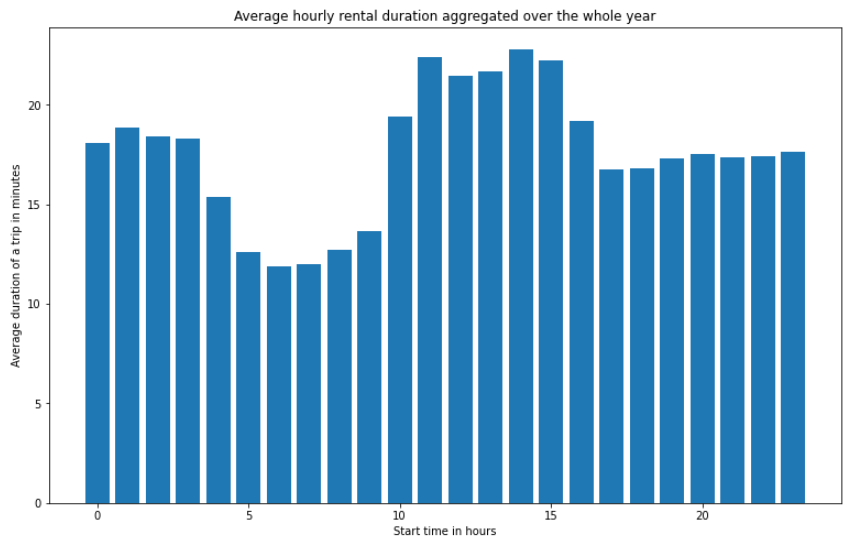
\includegraphics[width=0.8\linewidth]{./Figures/Duration_Fig_1.png}
    \caption{Average hourly rental duration aggregated over the whole year}
    \label{Duration_Fig_1}
\end{figure}

\subsection{KPI 4: Revenue}
\label{subsec:KPI4}

The revenue is the last KPI. The total revenue excluding subscriptions is 4656803 Dollar including subscriptions 8652803 Dollar \hyperref[fig_revenue_1]{(Figure 6)}. The revenue from subscribers can only be estimated, because they pay an annual subscription and we have not the number of subscribers nor the user IDs to calculate the numbers \hyperref[fig_revenue_1]{(Figure 6)}. The revenue from customers is directly depending on the number of trips from customers. Also, it is depending on the duration of the trips for both types of users as trips longer than 30 (customer) /45 minutes (subscriber) are paid by minute. Thus, the patterns observed for the usage of bike fleet and duration of trips apply to the revenue. The revenue from customers is volatile and peaks in summer while the revenue from the subscriptions is quite stable \hyperref[fig_revenue_2]{(Appendix Figure 7)}. Also, the mean revenue per trip is higher in summer than in winter due to the longer duration of trips in mean lead back to the weather. The mean revenue per trip per day is highest on the weekend \hyperref[fig_revenue_3]{(Appendix Figure 8)}. 

\begin{figure}[H]
    \centering
    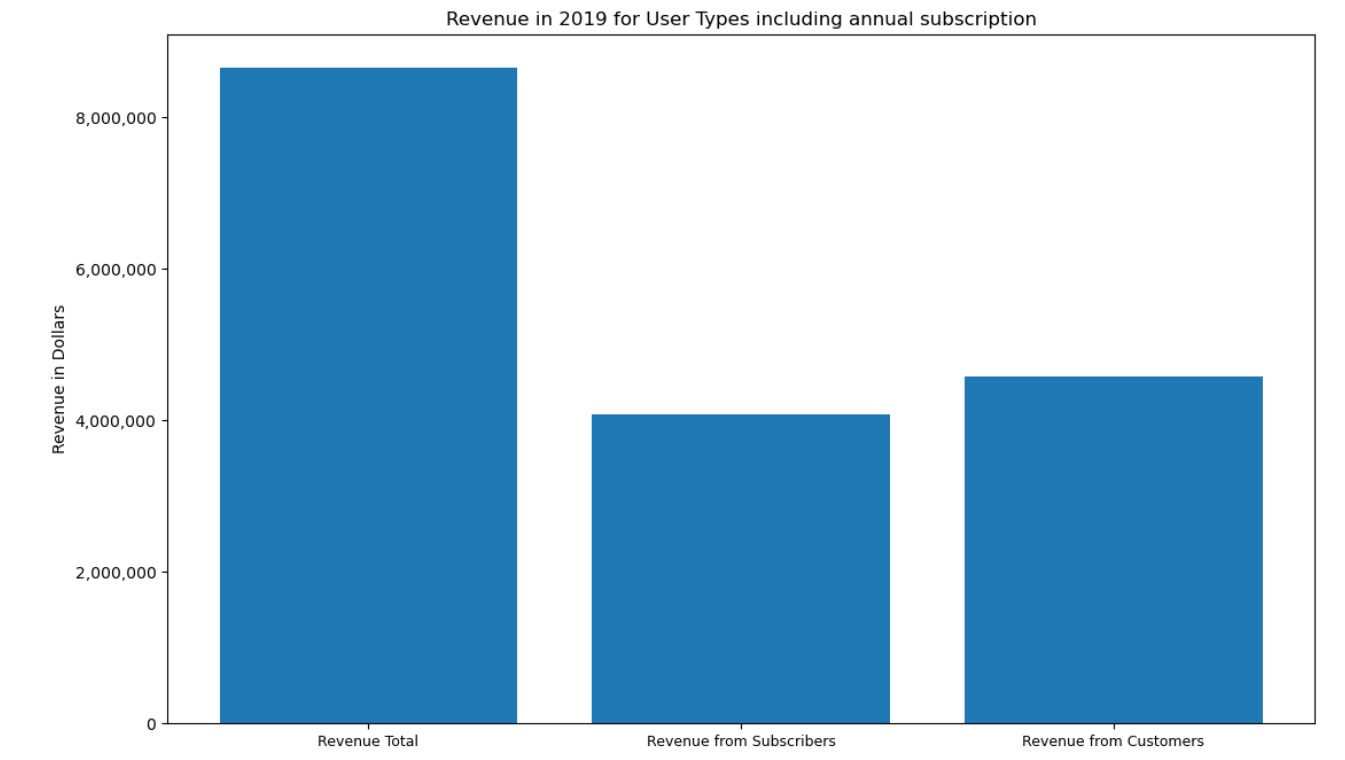
\includegraphics[width=0.7\linewidth]{./Figures/Revenue_annual.jpeg}
    \caption{Revenue in 2019 for User Types including annual subscription}
    \label{fig_revenue_1}
\end{figure}